% !TEX program = lualatex

\documentclass{article}
\usepackage[margin=5mm,paperwidth=10.5cm,paperheight=16.4cm]{geometry}
\usepackage{fontspec}
\usepackage{graphicx}
\usepackage{listings}
\usepackage{luacolor}
\usepackage[ngerman]{babel}
\usepackage{pgfpages}
\usepackage{tikz, tikzpagenodes}
\usepackage[a4,cam,cross]{crop}
\setmainfont{Antykwa Poltawskiego Light}

\definecolor{christmas}{HTML}{931111}
\renewcommand{\c}[1]{{\textcolor{christmas}{#1}}}

\pgfpagesdeclarelayout{christmas}{
    \edef\pgfpageoptionheight{\the\paperheight}
    \edef\pgfpageoptionwidth{\the\paperwidth}
    \edef\pgfpageoptionborder{0pt}
}{  \pgfpagesphysicalpageoptions{
        logical pages=2, physical height=29.7cm, physical width=21.0cm
    }\pgfpageslogicalpageoptions{2}{border shrink=\pgfpageoptionborder,
        resized width=10.5cm, resized height=16.4cm,
        center=\pgfpoint{.25\pgfphysicalwidth}{.5\pgfphysicalheight}
    }\pgfpageslogicalpageoptions{1}{border shrink=\pgfpageoptionborder,
        resized width=10.5cm, resized height=16.4cm,
        center=\pgfpoint{.75\pgfphysicalwidth}{.5\pgfphysicalheight}
    }
}

\begin{document}
\pgfpagesuselayout{christmas}\newgeometry{margin=2cm,top=3.3cm,bottom=3cm}%
\pagenumbering{gobble}\centering%
% www.fromoldbooks.org/Dalziel-RecordOfWork/pages/000-front-cover-good-words-1872
% Modified to better fit the image through image enhancement.
\begin{tikzpicture}[remember picture, overlay] \node[anchor=center]
    at (current page.center) {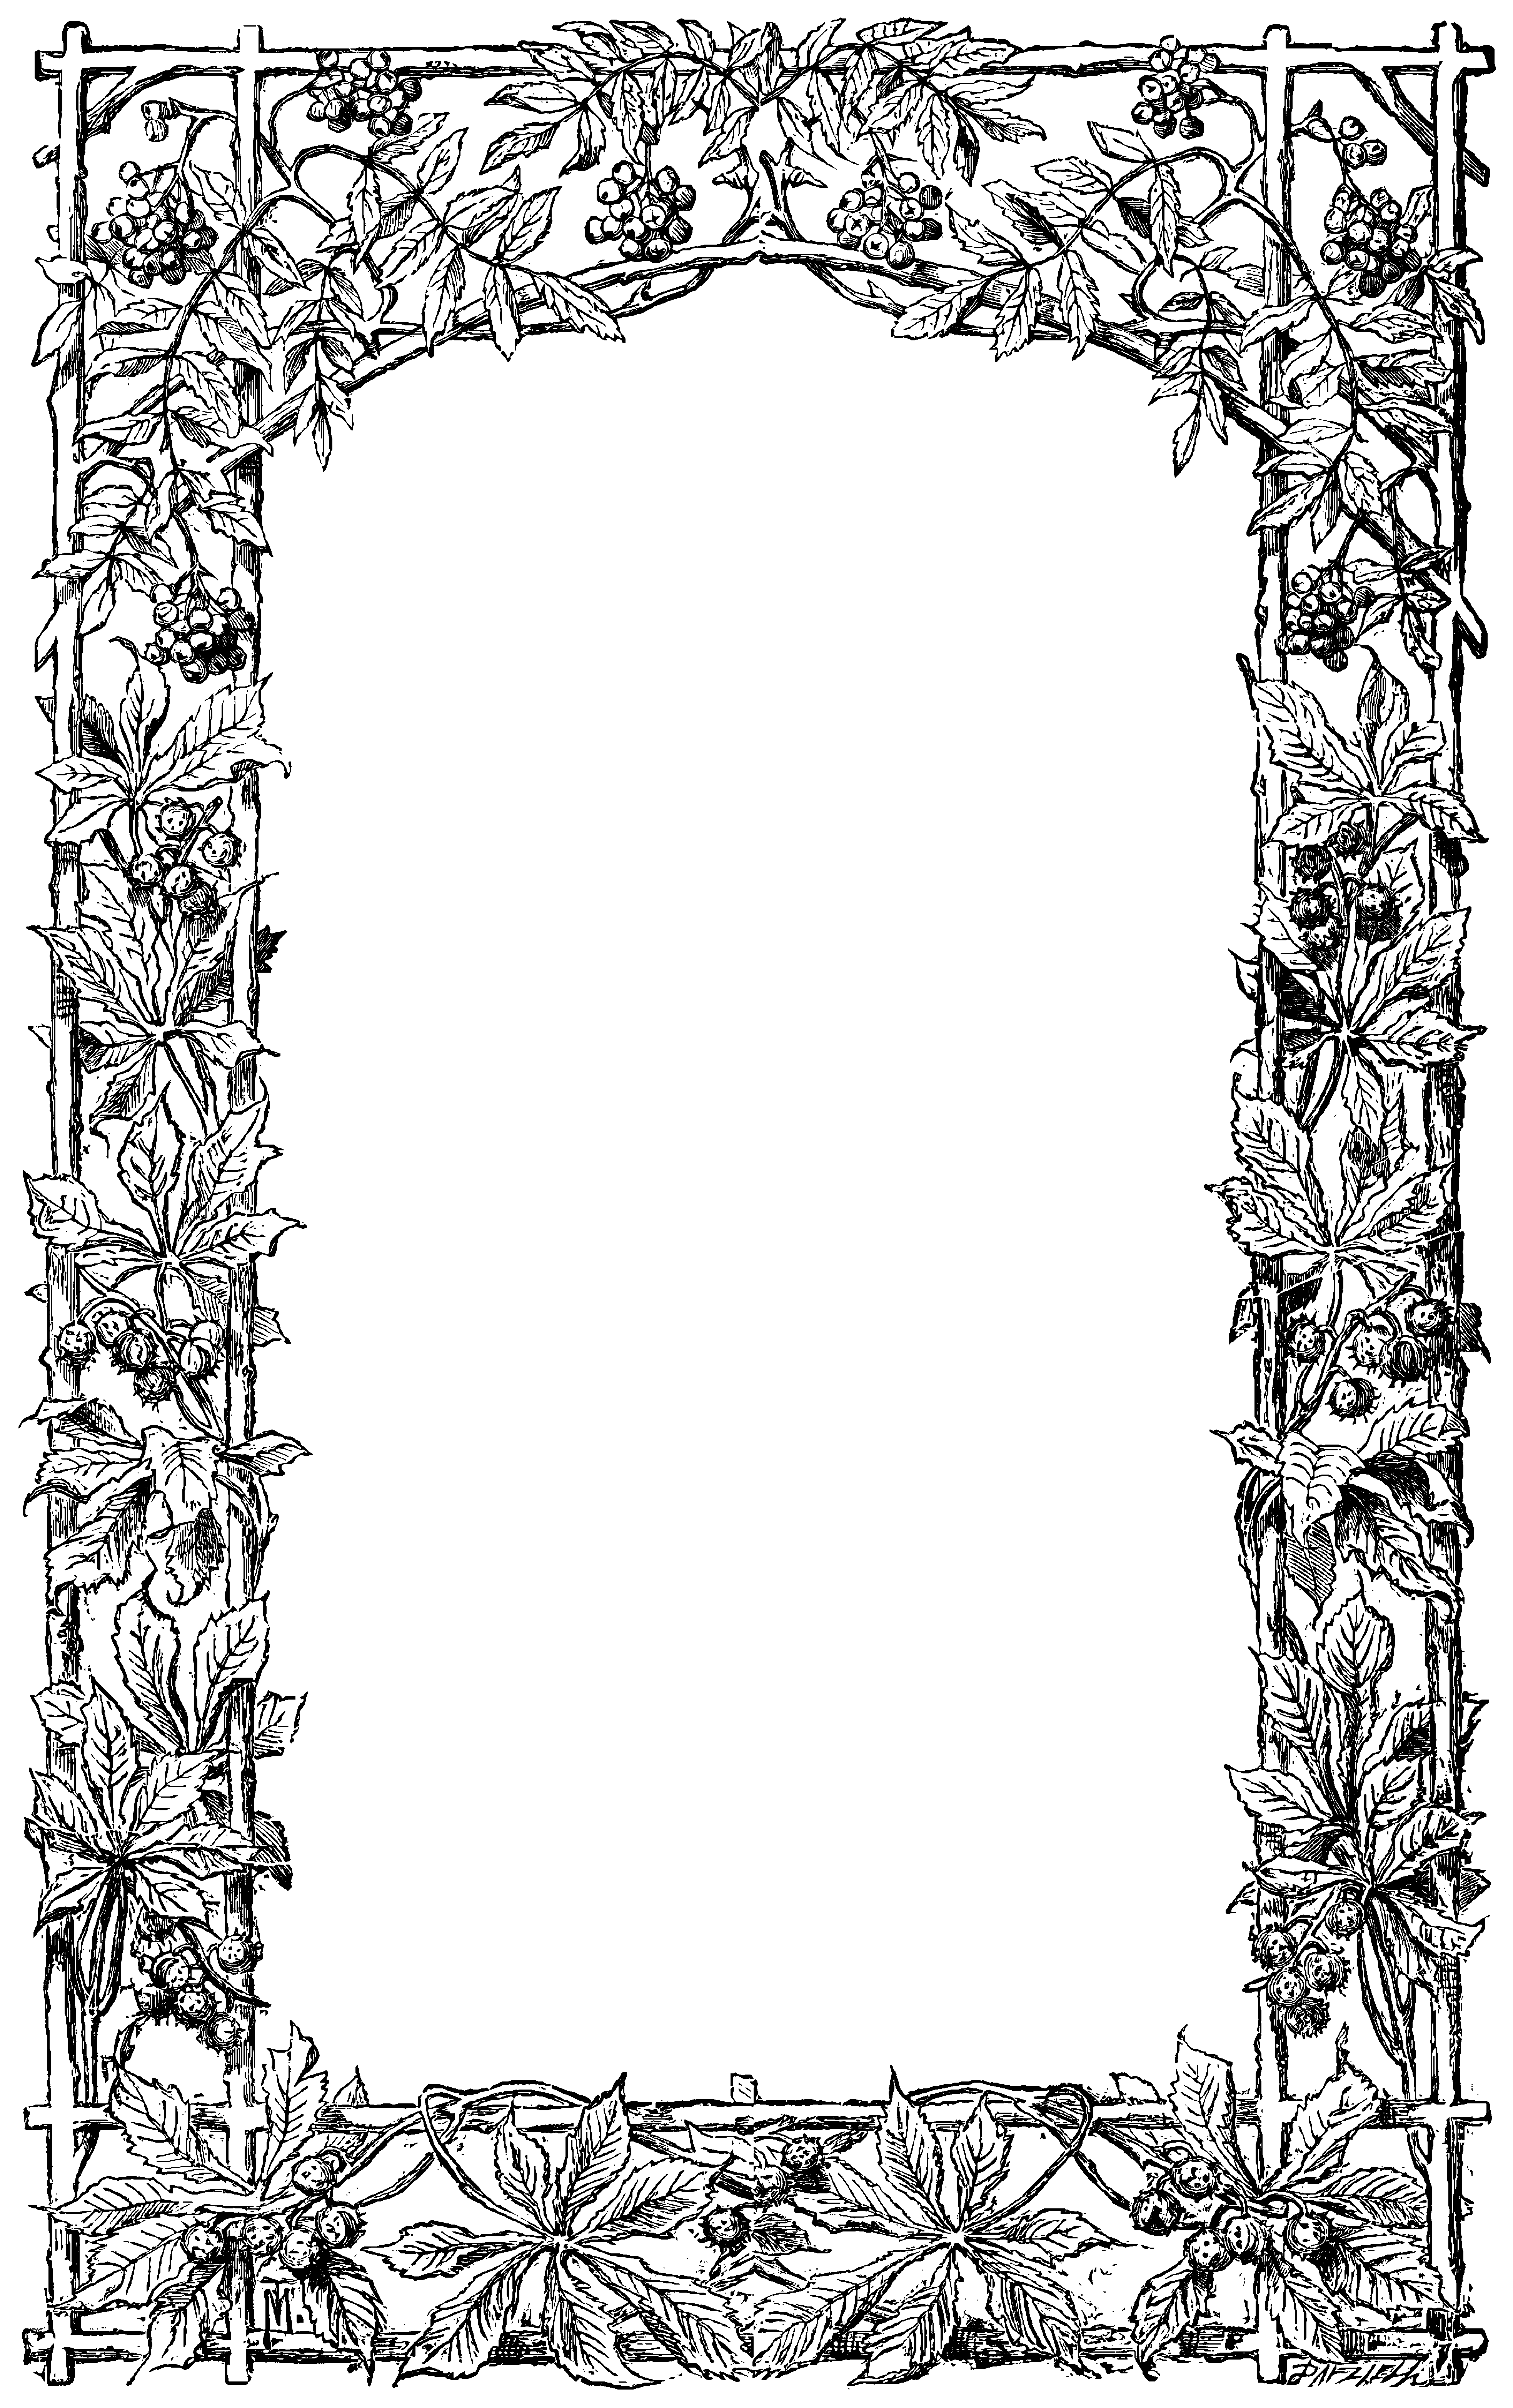
\includegraphics[width=.95\paperwidth]{frame}};
\end{tikzpicture} % You are being loved <3

{\LARGE \c{F}röhliche \c{W}eihnachten}\\\vfill
{\setmainfont{EB Garamond}\LARGE\textit{\c{\&}}}\\\vfill
{\large ein glückliches neues \c{J}ahr}\\[2mm]
{\large wünschen \c{H}ans und \c{F}lorentine.}\\

% https://www.oldbookillustrations.com/illustrations/brain-body/
% Manually thresholded, modified and edited
\vfill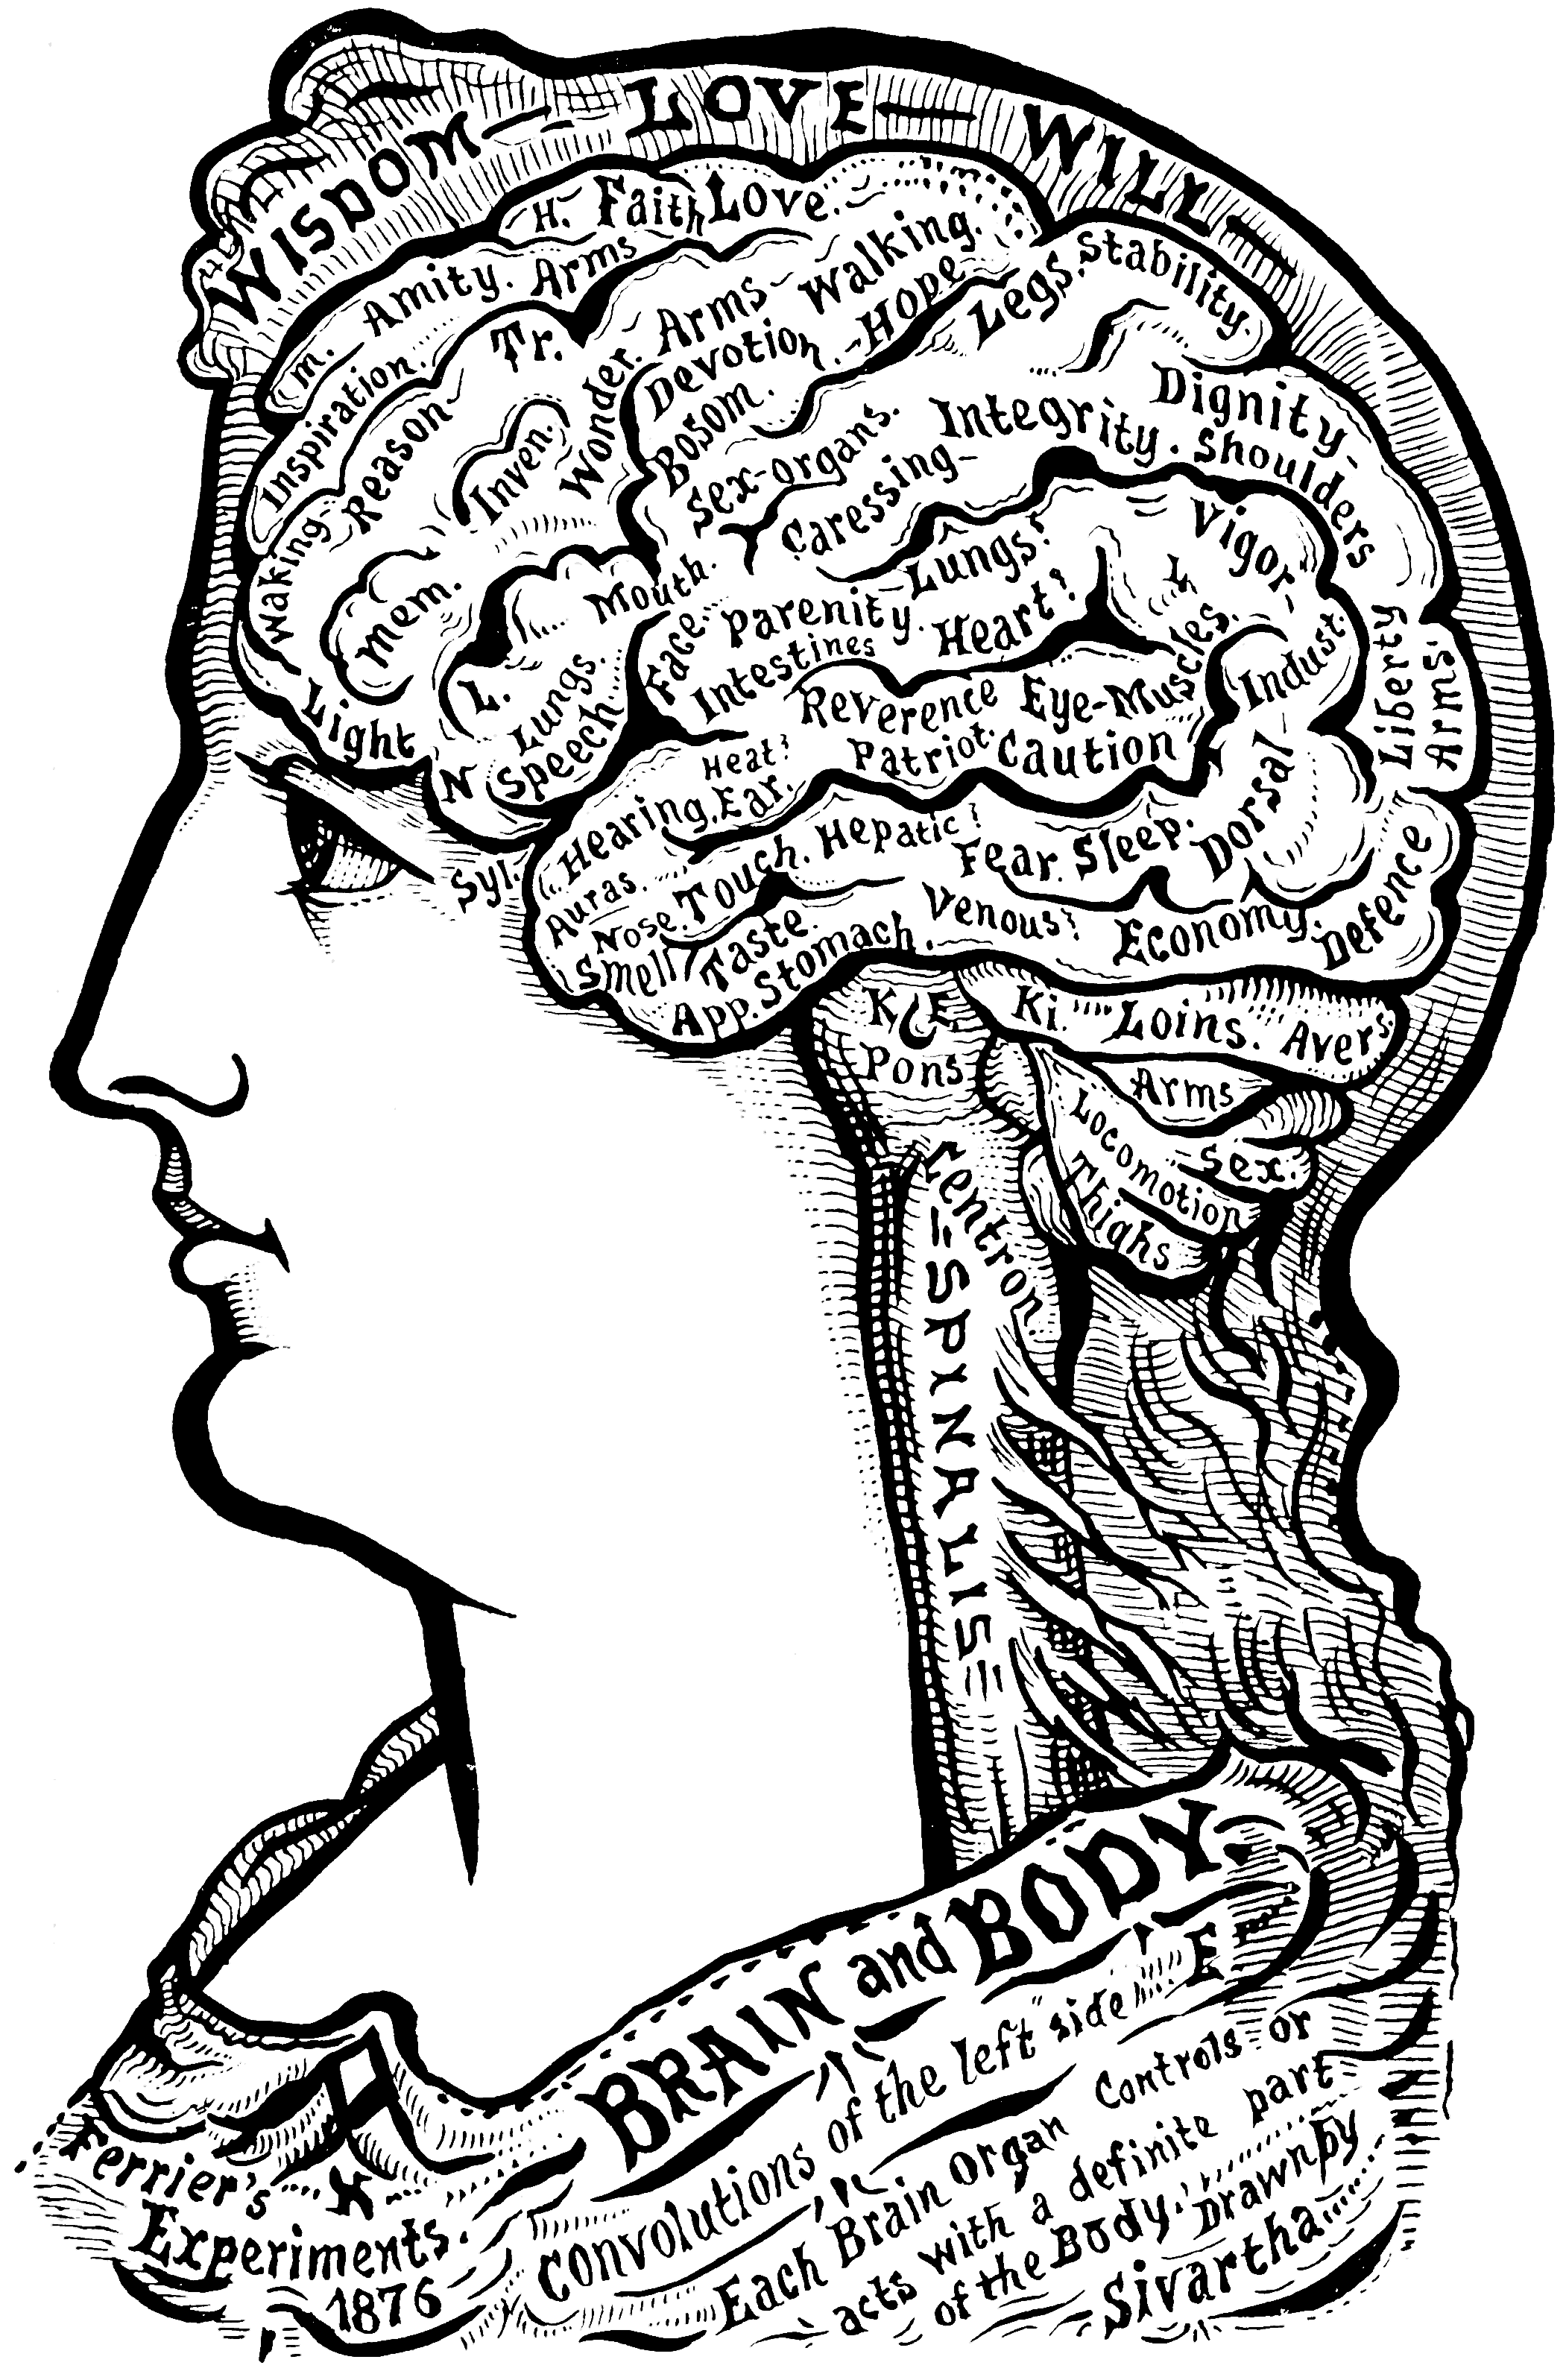
\includegraphics[height=4.75cm]{head}

\vfill\begin{minipage}[c]{.8\textwidth}\centering%
    \c{\glqq}Je kaputter die Welt draußen,
    desto heiler muss sie zu Hause sein.\c{\grqq}\\[2mm]
    \c{---}Reinhard Mey
\end{minipage}

\newpage\restoregeometry %%%%%%%%%%%%%%%%%%%%%%%%%%%%%%%%%%%%%%%%%%%%%
\lstinputlisting[
    language=TeX,morekeywords={begin,renewcommand,usepackage},
    basicstyle=\tiny\ttfamily,
    keywordstyle=\color{christmas},commentstyle=\color{darkgray}
]{christmas-card-2021.tex} % code page / back side
\vfill
{\small Typeset in Antykwa Półtawskiego and EB Garamond in \LaTeX.}
% The source code and the images are available on
% https://github.com/Kamik423/christmas-card-2021
\end{document}